% Cadence — Theory for Teammates (wrist tremor monitor + machine learning)
% ENGF0031 Scenario 2 "Smart Clothing".  Plain-English explainer for the team.
% Covers: tremor, frequency energy, machine learning, CNNs — from scratch.
% Sibling of cadence_theory.tex (that one is the ANKLE / freeze-of-gait version).
% Build:  tectonic cadence_theory_wrist.tex   (XeTeX engine, auto-downloads pkgs)
\documentclass[11pt]{article}

% ── Fonts (XeTeX / tectonic uses system fonts directly) ──────────────────────
\usepackage{fontspec}
\setmainfont{Helvetica Neue}
\setmonofont{Menlo}[Scale=0.88]

% ── Page geometry ────────────────────────────────────────────────────────────
\usepackage[a4paper, margin=1.9cm, top=1.7cm, bottom=1.8cm]{geometry}
\usepackage{microtype}
\usepackage{amsmath}
\usepackage{graphicx}
\usepackage{booktabs}
\usepackage{array}
\usepackage{enumitem}
\setlist{leftmargin=1.4em, itemsep=2pt, topsep=3pt}
\usepackage[most]{tcolorbox}
\usepackage{tikz}
\usetikzlibrary{positioning, arrows.meta, shapes.geometric, calc, fit,
                backgrounds, decorations.pathreplacing}
\usepackage{titlesec}
\usepackage{fancyhdr}

% ── Colour palette ───────────────────────────────────────────────────────────
\definecolor{teal}{HTML}{0E7C7B}
\definecolor{tealbg}{HTML}{E7F2F1}
\definecolor{amber}{HTML}{C9760D}
\definecolor{amberbg}{HTML}{FBEFDB}
\definecolor{ink}{HTML}{21302F}
\definecolor{muted}{HTML}{6B7B7A}
\definecolor{good}{HTML}{2E7D32}
\definecolor{bad}{HTML}{C0392B}
\definecolor{still}{HTML}{B9C3C3}
\definecolor{movec}{HTML}{7FC2C0}
\definecolor{tremc}{HTML}{EBB261}
\definecolor{plum}{HTML}{7A4E9E}
\definecolor{plumbg}{HTML}{F0EAF6}
\color{ink}

% ── Section styling ──────────────────────────────────────────────────────────
\titleformat{\section}
  {\Large\bfseries\color{teal}}{\makebox[1.1em][l]{\thesection}}{0pt}{}
\titleformat{\subsection}
  {\large\bfseries\color{ink}}{}{0pt}{}
\titlespacing*{\section}{0pt}{14pt}{6pt}
\titlespacing*{\subsection}{0pt}{9pt}{3pt}

% ── Footer ───────────────────────────────────────────────────────────────────
\pagestyle{fancy}\fancyhf{}
\renewcommand{\headrulewidth}{0pt}
\renewcommand{\footrulewidth}{0.4pt}
\fancyfoot[L]{\footnotesize\color{muted}Cadence — Theory for Teammates}
\fancyfoot[R]{\footnotesize\color{muted}\thepage}

% ── Callout boxes ────────────────────────────────────────────────────────────
\newtcolorbox{plain}{
  enhanced, breakable, colback=tealbg, frame hidden,
  borderline west={3pt}{0pt}{teal}, arc=2pt,
  left=10pt, right=10pt, top=7pt, bottom=7pt,
  before skip=7pt, after skip=7pt, fontupper=\normalsize}

\newtcolorbox{keyidea}{
  enhanced, breakable, colback=amberbg, frame hidden,
  borderline west={3pt}{0pt}{amber}, arc=2pt,
  left=10pt, right=10pt, top=7pt, bottom=7pt,
  before skip=7pt, after skip=7pt}

\newtcolorbox{mlbox}{
  enhanced, breakable, colback=plumbg, frame hidden,
  borderline west={3pt}{0pt}{plum}, arc=2pt,
  left=10pt, right=10pt, top=7pt, bottom=7pt,
  before skip=7pt, after skip=7pt}

% little inline "plain English" lead-in
\newcommand{\pe}{\textbf{\color{teal}In plain English:}\ }

% TikZ shared styles
\tikzset{
  blok/.style={rounded corners=3pt, draw=teal, line width=1pt, fill=tealbg,
               align=center, font=\small, inner sep=5pt},
  flow/.style={-{Latex[length=2.6mm]}, line width=1pt, draw=teal},
  flowA/.style={-{Latex[length=2.6mm]}, line width=1pt, draw=amber},
}

\begin{document}

% ════════════════════════════════════════════════════════════════════════════
% TITLE BLOCK
% ════════════════════════════════════════════════════════════════════════════
\begin{tcolorbox}[enhanced, colback=teal, colframe=teal, arc=4pt,
  left=16pt, right=16pt, top=13pt, bottom=13pt, boxrule=0pt]
  {\color{white}\Huge\bfseries Tremor, Frequency \&\\[2pt] Machine Learning}\\[5pt]
  {\color{white}\large How our wrist band measures a Parkinson's tremor
   \,---\, and how a neural network would do the same job. Explained from
   scratch, no physics needed.}\\[8pt]
  {\color{tealbg}\footnotesize ENGF0031 Scenario 2 \textbullet\ Cadence wrist
   monitor \quad\textbullet\quad A briefing for the team.}
\end{tcolorbox}

\vspace{2pt}
\noindent\small \textbf{How to use this.} Read it top to bottom and you can
explain the whole pipeline to anyone. Each section opens with the idea in one
breath, then a picture. Example numbers are marked \emph{illustrative} --- the
\emph{real} sensitivity/specificity come from our own wrist recording and go in
the worksheet, not here.
\normalsize

% ════════════════════════════════════════════════════════════════════════════
\section{What we are catching: a Parkinson's tremor}

Many people with Parkinson's disease have a \textbf{resting tremor}: the hand
shakes by itself, rhythmically, \emph{while it is resting} in the lap. It is
fast and small --- the hand trembles roughly \textbf{4 to 6 times every second}
--- and, oddly, it usually \emph{calms down} the moment the person reaches out
to do something on purpose. Clinicians track how strong and how frequent this
tremor is to see whether medication is working.

Our device, \textbf{Cadence}, is a small computer worn \textbf{on the wrist}
(think of a smartwatch). It watches the hand, measures how strong the tremor is,
and \emph{reports} it to a dashboard. That is all --- it does not buzz or shock
or correct anything. Measuring-and-reporting with no action back to the body is
called an \textbf{open loop} (a fitness tracker is open-loop; a thermostat that
switches the heater is \emph{closed}-loop).

\begin{plain}
\pe It is a thermometer for a tremor. A thermometer doesn't \emph{change} your
temperature, it just reports it honestly so a doctor can decide. Cadence reports
how much the hand is shaking at the tremor speed.
\end{plain}

\noindent The single most important fact for the whole project:

\begin{keyidea}
\textbf{A Parkinson's tremor has a \emph{fingerprint}: it is rhythmic, and it
happens at one particular speed (about 4--6 wiggles per second).} Random
fidgeting or reaching for a cup does not. So if we can measure ``how much
shaking is happening \emph{at the tremor speed}'', we can tell tremor apart from
ordinary life. Everything below is how we measure that one thing.
\end{keyidea}

% ════════════════════════════════════════════════════════════════════════════
\section{Frequency: shaking has a ``speed''}

\textbf{Frequency} just means \emph{how many wiggles happen per second}. We
measure it in \textbf{hertz (Hz)}: 5\,Hz means back-and-forth five times a
second. Slow wiggles are a low frequency; fast wiggles are a high frequency.

\pe Think of sound. A deep bass note is a slow vibration (low frequency); a high
treble note is a fast vibration (high frequency). A tremor is like a single,
steady note your wrist keeps humming at about 5\,Hz.

Here is the trick that makes the whole field possible. \textbf{Any messy,
wiggly signal can be seen as a stack of pure, simple wiggles of different speeds,
all added together.} Pull them back apart and you can ask ``how much of each
speed is in here?'' That ``how much of each speed'' picture is called a
\textbf{spectrum} (or \emph{power spectrum}).

\pe A spectrum is the bar-graph equaliser on a music app. Music is many notes
mixed together; the equaliser shows how loud each pitch is. A spectrum does the
same for your wrist: it shows how strong the shaking is at each speed.

\begin{center}
\resizebox{0.92\linewidth}{!}{%
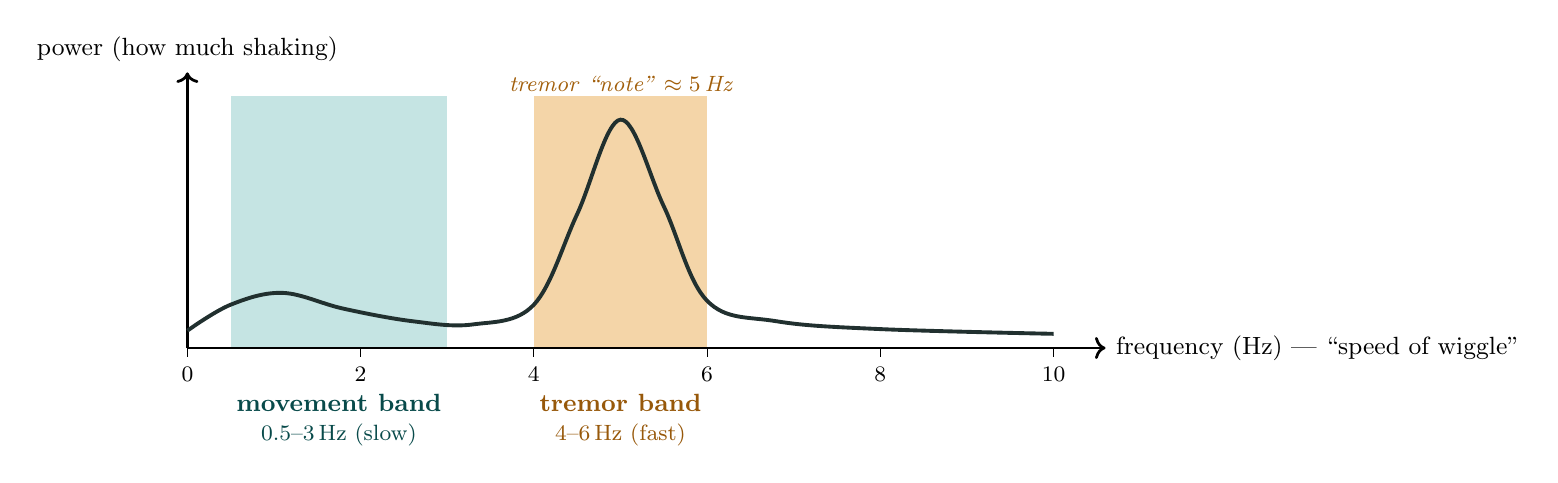
\begin{tikzpicture}[x=11mm, y=10mm]
  % bands behind
  \fill[movec!45] (0.5,0) rectangle (3,3.2);
  \fill[tremc!55] (4,0) rectangle (6,3.2);
  % axes
  \draw[->, line width=1pt] (0,0) -- (10.6,0) node[right, font=\small]{frequency (Hz) --- ``speed of wiggle''};
  \draw[->, line width=1pt] (0,0) -- (0,3.5) node[above, font=\small]{power (how much shaking)};
  \foreach \xx in {0,2,4,6,8,10} \draw (\xx,0) -- (\xx,-0.12) node[below, font=\footnotesize]{\xx};
  % the spectrum curve: small low-freq tail + sharp tremor peak near 5 Hz
  \draw[line width=1.4pt, ink] plot[smooth, tension=0.6] coordinates
    {(0,0.22)(0.5,0.55)(1.1,0.7)(1.8,0.5)(2.6,0.34)(3.3,0.3)
     (4.0,0.55)(4.5,1.7)(5.0,2.9)(5.5,1.8)(6.0,0.6)(6.8,0.34)(8,0.24)(10,0.18)};
  % labels
  \node[font=\small\bfseries, text=teal!60!black] at (1.75,-0.7) {movement band};
  \node[font=\footnotesize, text=teal!60!black] at (1.75,-1.1) {0.5--3\,Hz (slow)};
  \node[font=\small\bfseries, text=amber!75!black] at (5.0,-0.7) {tremor band};
  \node[font=\footnotesize, text=amber!75!black] at (5.0,-1.1) {4--6\,Hz (fast)};
  \node[font=\footnotesize\itshape, text=amber!80!black] at (5.0,3.35) {tremor ``note'' $\approx5$\,Hz};
\end{tikzpicture}}
\\[2pt]
{\footnotesize\color{muted}(Illustrative spectrum of a resting hand with a
tremor: a sharp bump sits in the 4--6\,Hz band. Voluntary movement instead puts
its energy down in the slow 0.5--3\,Hz band.)}
\end{center}

% ════════════════════════════════════════════════════════════════════════════
\section{Energy in a band: turning shaking into ONE number}

We don't need the whole spectrum --- we only care about \emph{one} part of it:
the \textbf{4--6\,Hz tremor band}. We add up how strong the shaking is across
just that band and call it the \textbf{tremor power}: one number that means
``how much tremor-speed shaking is going on right now''. Big number $=$ strong
tremor; near-zero $=$ a calm hand.

How does a tiny battery chip compute that, live, without a maths
supercomputer? Two cheap steps:

\begin{enumerate}
  \item \textbf{A band-pass filter --- a gatekeeper.} A filter is a piece of
        maths that lets some wiggle-speeds through and blocks the rest. Ours is
        a \emph{band-pass} filter tuned to 4--6\,Hz: it throws away slow drift
        and arm-swinging (too slow) \emph{and} fast electrical noise (too fast),
        and keeps only tremor-speed wiggle.
        \pe It's like noise-cancelling headphones set to keep \emph{only} a
        5\,Hz hum and mute everything else.
  \item \textbf{Square and sum --- measure the leftover.} Whatever survives the
        filter, we \emph{square} each sample (squaring makes every value
        positive and makes big swings count much more than small ones --- that
        is what ``energy'' means) and add them all up. The total is the tremor
        power.
\end{enumerate}

\begin{center}
\begin{tcolorbox}[enhanced, colback=white, colframe=teal, boxrule=1pt, arc=3pt,
   width=0.9\linewidth, halign=center, top=8pt, bottom=8pt]
  \large$\displaystyle
  \text{tremor power}=\sum_{\text{samples in the window}}
        \big(\text{wiggle left after the 4--6\,Hz filter}\big)^{2}$
\end{tcolorbox}
\end{center}

\noindent We compute this over a \textbf{4-second window} of data and refresh it
every \textbf{2 seconds}, so the dashboard updates twice as often as the window
is long. (Four seconds is long enough to \emph{see} a 5\,Hz rhythm clearly; you
can't judge a rhythm from a single instant.)

\begin{plain}
\pe A band-pass filter $+$ ``square and add up'' is the cheap way to ask ``how
loud is the 4--6\,Hz band?'' without computing the whole equaliser. It's a few
multiplications per sample --- easy for a coin-cell chip, and exactly what our
firmware (\texttt{cpx\_tremor\_monitor.ino}) does.
\end{plain}

\subsection*{Two small honesty checks before we believe it}
\begin{itemize}
  \item \textbf{Is the hand actually at rest? (the rest gate.)} A
        \emph{resting} tremor only counts when the hand is resting. If the
        person is busy waving or walking, there's lots of slow 0.5--3\,Hz
        movement --- so we check that band too, and if it's high we say
        ``moving, ignore the tremor reading'' rather than cry wolf.
  \item \textbf{Is it sustained? (debounce.)} One odd 2-second window shouldn't
        flip the verdict. We require \textbf{2 windows in a row} over the line
        to declare ``tremor present'', and 2 clear ones to declare it gone. That
        stops the readout flickering.
\end{itemize}

\subsection*{Where the score comes from}
To grade the device we set a \textbf{threshold} (a line) on the tremor power and,
window by window, compare what the device says to the truth. That gives the two
headline numbers the worksheet asks for:
\textbf{sensitivity} (``of the real tremor windows, how many did we catch?'')
and \textbf{specificity} (``of the calm/normal windows, how many did we
correctly leave alone?''). We report those two, \emph{not} ``accuracy'', because
tremor windows are rare --- a lazy detector that says ``never'' would score high
accuracy while catching nothing.

% ════════════════════════════════════════════════════════════════════════════
\section{Machine learning: a different way to make the rule}

Everything above is a \textbf{hand-written rule}: \emph{we}, the humans, studied
the problem and decided ``filter to 4--6\,Hz, measure the power, compare to a
line''. There is a completely different philosophy, and it is what people mean
by \textbf{machine learning (ML)}.

\begin{center}
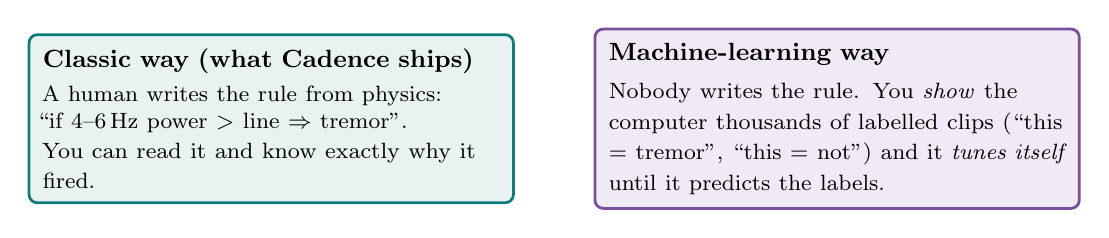
\begin{tikzpicture}[node distance=6mm]
  \node[blok, text width=58mm, align=left, fill=tealbg, draw=teal]
    (a) {\textbf{Classic way (what Cadence ships)}\\[3pt]\footnotesize
         A human writes the rule from physics:\\
         ``if 4--6\,Hz power $>$ line $\Rightarrow$ tremor''.\\
         You can read it and know exactly why it fired.};
  \node[blok, text width=58mm, align=left, right=10mm of a,
        fill=plumbg, draw=plum]
    (b) {\textbf{Machine-learning way}\\[3pt]\footnotesize
         Nobody writes the rule. You \emph{show} the computer thousands of
         labelled clips (``this $=$ tremor'', ``this $=$ not'') and it
         \emph{tunes itself} until it predicts the labels.};
\end{tikzpicture}
\end{center}

\pe Teaching a kid the word ``dog'' the classic way means listing rules: four
legs, fur, a tail\dots\ (and a cat sneaks through). The machine-learning way is
to show them hundreds of photos labelled ``dog / not dog'' until they just
\emph{get} it. ML learns from examples, not from a rulebook.

How does it ``tune itself''? Inside the model are thousands of little numbers
called \textbf{weights} --- think tiny knobs. \textbf{Training} is a loop: the
model guesses, we compare its guess to the true label, and we nudge every knob a
hair in the direction that would have made the guess better. Do that over
millions of examples and the knobs settle into a setting that works.

\begin{mlbox}
\textbf{The trade.} ML can learn patterns a human would never think to write
down --- but it needs \emph{a lot} of labelled examples to learn from, more
memory and computing power to run, and it can't easily \emph{tell} you why it
decided something. A hand-written rule is the opposite: limited, but tiny,
instant, and fully explainable.
\end{mlbox}

% ════════════════════════════════════════════════════════════════════════════
\section{CNN: a pattern-finder for signals}

A \textbf{neural network} is just a big stack of those weighted knobs arranged in
layers, where each layer's output feeds the next. A \textbf{convolutional neural
network (CNN)} is a \emph{special} kind that is brilliant at finding \textbf{local
patterns} in grid-shaped data --- pixels in an image (a 2-D grid) or, for us,
\textbf{samples over time} (a 1-D grid). For accelerometer signals we'd use a
\emph{1-D} CNN.

The key move is the \textbf{convolution}: take a small ``pattern detector''
(called a \textbf{kernel} or \textbf{filter}) and \emph{slide it along} the
signal, scoring how well the signal matches that pattern at every position.
Where the pattern appears, the score spikes.

\pe A convolution is a little transparent stencil you slide across the signal.
Wherever the shape underneath matches the stencil, it lights up. Slide a
``5\,Hz burst'' stencil along a wrist trace and it lights up exactly on the
tremor.

\begin{center}
\resizebox{0.95\linewidth}{!}{%
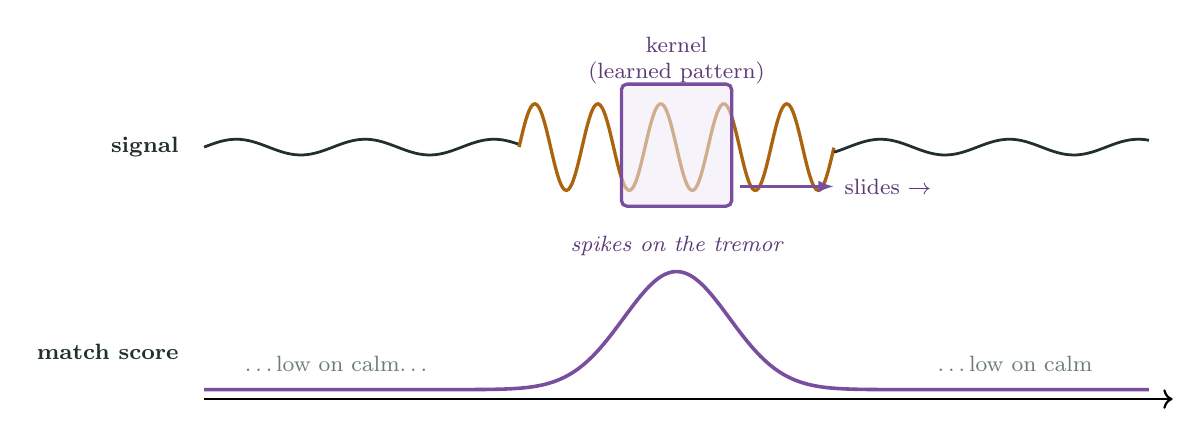
\begin{tikzpicture}[x=10mm, y=10mm]
  % ---- input signal: calm, then a 5 Hz burst, then calm ----
  \node[font=\footnotesize\bfseries, text=ink, anchor=east] at (-0.2,2.2){signal};
  \draw[line width=1pt, ink, samples=80, smooth] plot[domain=0:4]
        (\x,{2.2+0.10*sin(220*\x)});
  \draw[line width=1.2pt, amber!85!black, samples=160, smooth] plot[domain=4:8]
        (\x,{2.2+0.55*sin(450*(\x-4))});
  \draw[line width=1pt, ink, samples=80, smooth] plot[domain=8:12]
        (\x,{2.2+0.10*sin(220*\x)});
  % ---- sliding kernel window (over the burst) ----
  \draw[plum, line width=1.2pt, fill=plumbg, fill opacity=0.55, rounded corners=2pt]
        (5.3,1.45) rectangle (6.7,3.0);
  \node[font=\footnotesize, text=plum!75!black, align=center] at (6.0,3.3)
        {kernel\\(learned pattern)};
  \draw[-{Latex[length=2mm]}, plum, line width=1pt] (6.8,1.7) -- (8.0,1.7)
        node[right, font=\footnotesize, text=plum!75!black]{slides $\rightarrow$};
  % ---- output: match score, low on calm, hump on burst ----
  \node[font=\footnotesize\bfseries, text=ink, anchor=east] at (-0.2,-0.4){match score};
  \draw[->, line width=0.8pt] (0,-1) -- (12.3,-1);
  \draw[line width=1.3pt, plum, samples=120, smooth] plot[domain=0:12]
        (\x,{-1+0.12+1.5*exp(-((\x-6)*(\x-6))/0.9)});
  \node[font=\footnotesize\itshape, text=plum!75!black] at (6,0.95){spikes on the tremor};
  \node[font=\footnotesize, text=muted] at (1.7,-0.55){\dots low on calm\dots};
  \node[font=\footnotesize, text=muted] at (10.3,-0.55){\dots low on calm};
\end{tikzpicture}}
\\[2pt]
{\footnotesize\color{muted}(A convolution slides a small learned pattern across
the signal and reports how well it matches at each point. A real CNN stacks many
such detectors.)}
\end{center}

A CNN stacks these: the first layer's kernels find tiny features (a short
up-down wiggle); the next layer combines those into bigger ideas (``a sustained
5\,Hz burst lasting two seconds''); a final layer turns that into a verdict,
``tremor / not''. Crucially, \textbf{it learns the kernels itself} from labelled
data --- nobody hand-draws the stencils.

\begin{mlbox}
\textbf{The punchline that connects everything.} Our hand-built 4--6\,Hz
band-pass filter \emph{is} a convolution --- one stencil, designed by us from
physics. A 1-D CNN would \emph{learn a whole stack} of stencils from data. Fed
enough labelled wrist recordings, it might rediscover ``watch the 4--6\,Hz
band'' on its own \emph{and} pick up subtler cues (how the tremor ramps up, how
it differs from a shiver) that a single fixed filter misses. Same family of
maths --- one hand-tuned, one learned.
\end{mlbox}

% ════════════════════════════════════════════════════════════════════════════
\section{So which does Cadence use --- and why?}

We ship the \textbf{hand-built filter}, not a CNN. Here is the honest
side-by-side so the team can defend the choice:

\begin{center}
\renewcommand{\arraystretch}{1.35}
\begin{tabular}{>{\raggedright\arraybackslash}p{4.3cm}
                >{\raggedright\arraybackslash}p{5.4cm}
                >{\raggedright\arraybackslash}p{5.4cm}}
\toprule
& \textbf{\color{teal}Hand-built filter} \newline (what we ship)
& \textbf{\color{plum}1-D CNN} \newline (the ML alternative)\\
\midrule
How the rule is made & A human, from physics & Learned from labelled data\\
Needs training data?  & No & Yes --- and lots of it\\
Runs on the coin-cell CPX? & Yes, a few sums per sample & Heavy: needs more memory \& compute\\
Can it explain itself?     & Fully (``4--6\,Hz power $>$ line'') & Mostly a black box\\
Best when\dots             & you understand the signal, have little data, and must justify every reading & you have lots of labelled data and want to catch subtle patterns\\
\bottomrule
\end{tabular}
\end{center}

\noindent For a \textbf{one-week clinical prototype} the filter wins on every
axis that matters to us: we have very little labelled tremor data, the code must
run on the tiny Circuit Playground, and a clinician has to \emph{trust} and
justify every number it reports --- which is easy when the rule is ``power in
the tremor band crossed a line''. The CNN is the honest \emph{``given more data
and time''} upgrade, not a corner we cut.

\begin{plain}
\pe We didn't avoid machine learning because it's hard --- we chose the simpler
tool because it's the \emph{right} one for a tiny, explainable, low-data medical
monitor. Knowing \emph{when not} to reach for the fancy method is itself good
engineering.
\end{plain}

% ════════════════════════════════════════════════════════════════════════════
\section{One-page cheat sheet}

\begin{tcolorbox}[enhanced, colback=white, colframe=teal, boxrule=1pt, arc=3pt,
   left=12pt, right=12pt, top=9pt, bottom=9pt]
\begin{description}[leftmargin=9.2em, style=nextline, font=\bfseries\color{teal}]
  \item[Resting tremor] the hand shaking by itself at rest, about 4--6 times a
        second; calms during deliberate movement. This is what we measure.
  \item[Frequency (Hz)] how many wiggles per second. Movement $=$ slow
        (0.5--3\,Hz); tremor $=$ fast (4--6\,Hz).
  \item[Spectrum] the ``equaliser'' picture: how much shaking sits at each
        frequency.
  \item[Band-pass filter] a gatekeeper that keeps only 4--6\,Hz wiggle and
        blocks the rest.
  \item[Tremor power] filter to 4--6\,Hz, square each sample, add them up. One
        number for ``how much tremor''.
  \item[Window] 4\,s of data, refreshed every 2\,s, so the readout updates often
        with enough context to judge a rhythm.
  \item[Rest gate] ignore the tremor reading while the hand is actively moving
        (lots of slow-band power).
  \item[Debounce] need 2 windows in a row to change the verdict; stops flicker.
  \item[Sensitivity] catch rate: of real tremor windows, how many we caught.
  \item[Specificity] leave-alone rate: of calm windows, how many we correctly
        ignored. (We report these two, not ``accuracy''.)
  \item[Machine learning] don't hand-write the rule --- learn it from thousands
        of labelled examples by nudging internal ``knobs'' (weights).
  \item[CNN] a network that finds patterns by sliding small learned ``stencils''
        (kernels) across the data. Our fixed filter is one stencil; a CNN learns
        a stack of them.
\end{description}
\end{tcolorbox}

\vfill
\noindent{\footnotesize\color{muted}Built for ENGF0031 Scenario 2 ``Smart
Clothing''. This is a teammate explainer; the spectrum and CNN sketches are
illustrative. Real device performance (sensitivity / specificity) comes from our
own wrist recording and is reported in the accuracy worksheet, not here. The
ankle / freeze-of-gait version of this theory lives in \texttt{cadence\_theory.tex}.}

\end{document}
